\documentclass[aspectratio=169, pdf, 8pt, unicode]{beamer}
\usepackage[american,russian]{babel}
\usepackage[default]{sourcesanspro}
\usepackage{tikz}
\usepackage{tikzscale}
\usepackage{float}
\usepackage{graphicx}
\usepackage{pgfplotstable}
\usepackage{caption}
\usepackage{amsmath}
\usepackage{amssymb}
\usepackage{setspace}
\usepackage{fancyvrb}

\usepackage[backend=biber,bibencoding=utf8,sorting=none,maxcitenames=2,style=gost-numeric]{biblatex}
\addbibresource{src/references.bib}

\usetikzlibrary{chains,fit,shapes,arrows.meta}

\DeclareCaptionLabelFormat{gostfigure}{Рисунок #2}
\captionsetup[table]{labelsep=endash,justification=justified,singlelinecheck=false,font=normalsize,skip=0pt} 
\captionsetup[figure]{labelformat=gostfigure,labelsep=endash,justification=centering,singlelinecheck=false,font=normalsize} 
\pgfplotsset{compat=1.9}

\mode<presentation> {
\usetheme{Madrid}
}

\setbeamerfont{institute}{size=\normalsize}
\setbeamertemplate{itemize/enumerate body begin}{\large}
\setbeamertemplate{itemize/enumerate subbody begin}{\tiny}

\title[Теория и практика многопоточного программирования]{Теория и практика многопоточного программирования\\ \vspace{0.5cm}Семинар 1}

\author{Неганов Алексей}

\institute[МФТИ]{
    Московский физико-технический институт (национальный исследовательский университет)\\
    Кафедра теоретической и прикладной информатики\\
}

\date{Москва 2020}

\setbeamertemplate{caption}[numbered]

\begin{document}

\begin{frame}
\titlepage
\end{frame}


\begin{frame}
\frametitle{Ожидаемые знания}
	\begin{itemize}
		\setlength\itemsep{4em}
		\item Основы теории ОС
		\item Основы архитектуры компьютера
		\item Языки C и С++
	\end{itemize}
\end{frame}

\begin{frame}
\frametitle{Горизонты}
	\begin{itemize}
		\item Oсновные концепции параллельного программирования c разделяемой памятью
		\item Базовые сведения об архитектуре многопроцессорных компьютеров
		\item Декомпозиция задач
		\item Синхронизация
		\item Разбор распространённых проблем
		\item Разбор работы с потоками и процессами ОС
		\item Ввод-вывод в многопоточной системе
		\item Реализация важнейших примитивов и алгоритмов на языках C и C++
		\item Исследование поведения паралельных программ под нагрузкой
	\end{itemize}
	Дополнительно:
	\begin{itemize}
		\item Демонстрация некоторых решений на языке Go
		\item OpenMP
		\item Проблемы параллельного исполнения транзакций БД
		\item ...
	\end{itemize}
\end{frame}

\begin{frame}[fragile]
\frametitle{Многозадачность}
\begin{figure}[H]
      \centering
      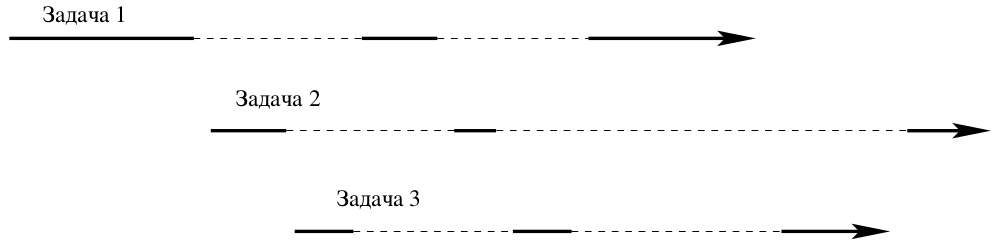
\includegraphics[width=0.6\textwidth]{fig/multitasking.png}
      \caption{Одновременное выполнение задач на одном процессоре}
\end{figure}
\begin{figure}[H]
      \centering
      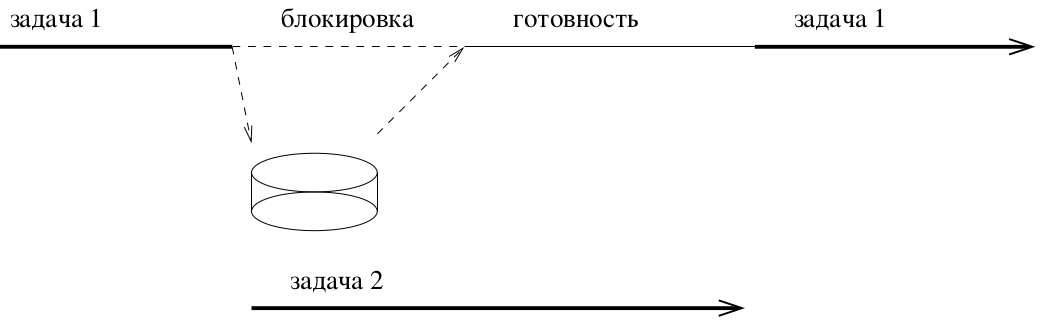
\includegraphics[width=0.6\textwidth]{fig/multitasking_io.png}
      \caption{Пакетный режим}
\end{figure}
\end{frame}

\begin{frame}[fragile]
\frametitle{Классификация архитектур ЭВМ}
\begin{figure}[H]
      \centering
      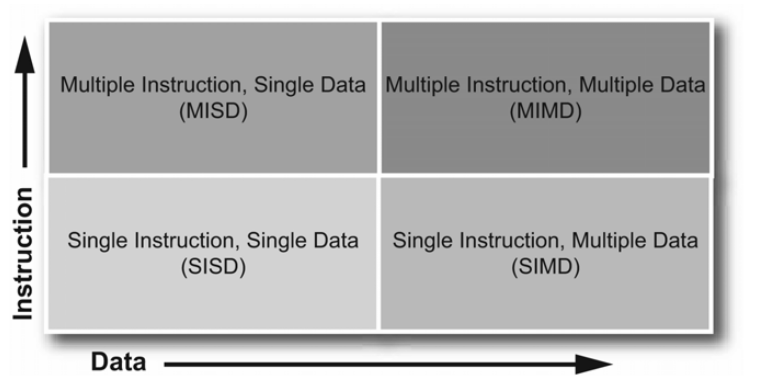
\includegraphics[width=0.75\textwidth]{fig/flinn.png}
      \caption{Таксономия Флинна}
\end{figure}
\end{frame}

\begin{frame}[fragile]
\frametitle{Атомарность операций}
Чему может оказаться равен \texttt{x}?
\begin{figure}[H]
\centering
\begin{BVerbatim}
int x = 17;

process foo { 
    x++;
}

process bar { 
    x++;
}

process baz { 
    x++;
}
\end{BVerbatim}
\end{figure}
\end{frame}

\begin{frame}[fragile]
\frametitle{Атомарность операций}
\begin{figure}[H]
	  \centering
      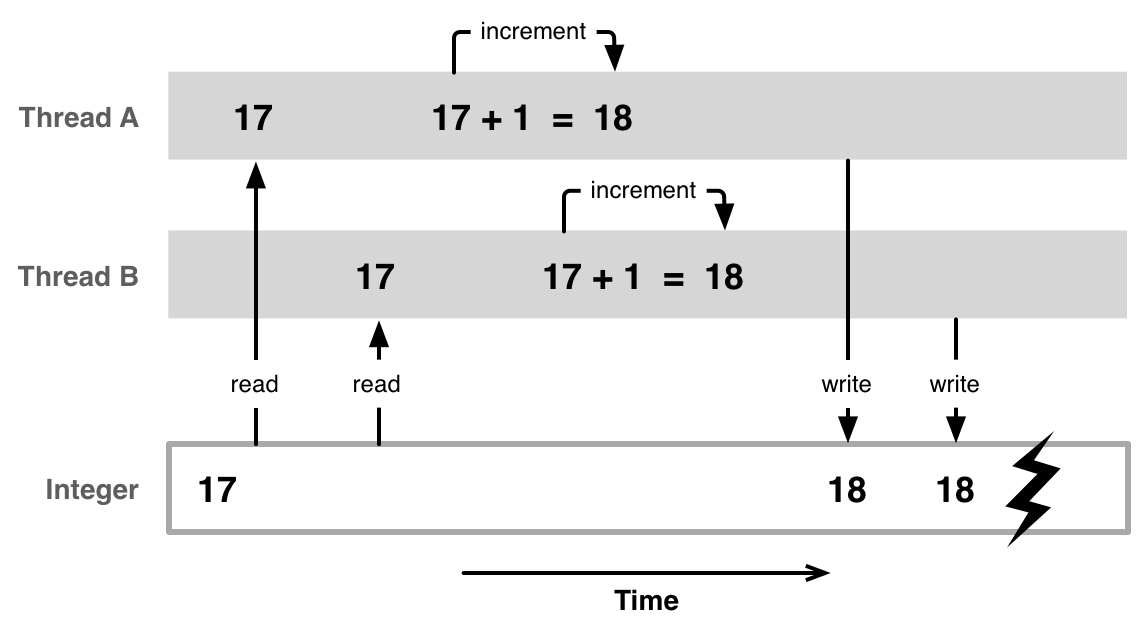
\includegraphics[width=0.6\textwidth]{fig/race-condition-inc.png}
      \caption{Иллюстрация состояния гонки для оператора инкремента}
\end{figure}
\end{frame}

\begin{frame}[fragile]
\frametitle{Связность памяти}
\begin{figure}[H]
      \centering
      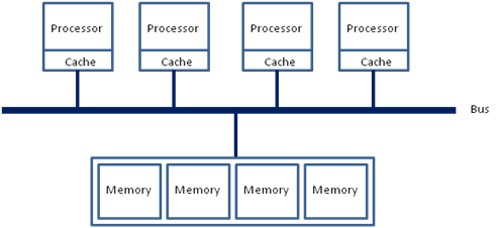
\includegraphics[width=0.5\textwidth]{fig/smp.png}
      \caption{Соединение типа SMP}
\end{figure}
\end{frame}

\begin{frame}[fragile]
\frametitle{Связность памяти}
\begin{figure}[H]
      \centering
      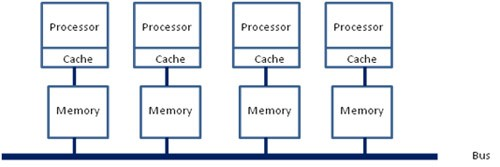
\includegraphics[width=0.5\textwidth]{fig/numa.jpg}
      \caption{Соединение типа NUMA}
\end{figure}
\end{frame}

\begin{frame}[fragile]
\frametitle{Связность памяти}
\begin{figure}[H]
      \centering
      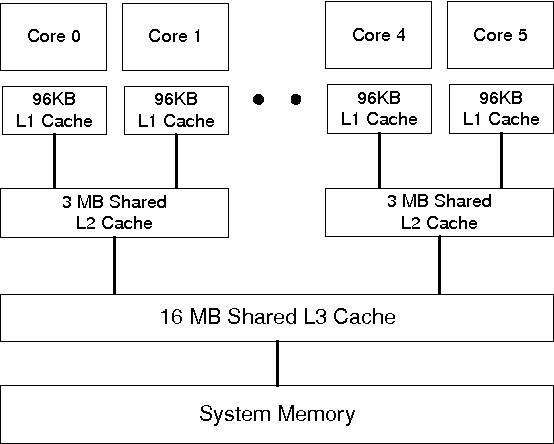
\includegraphics[width=0.4\textwidth]{fig/memory-hierarchy.png}
      \caption{Иерархия памяти для многоядерной SMP-системы}
\end{figure}
\end{frame}

\begin{frame}[fragile]
\frametitle{Коварный кэш}
Может ли выполниться \texttt{assert()}?
\begin{figure}[H]
\centering
\begin{BVerbatim}
int a = 0;
int b = 0;

void foo(void) {
      a = 1;
      b = 1;
}

void bar(void) {
      while(b == 0);
      assert(a == 1);
}
\end{BVerbatim}
\end{figure}
\end{frame}

\begin{frame}[fragile]
\frametitle{Коварный кэш}
Может ли выполниться \texttt{assert()}?
\begin{figure}[H]
\centering
\begin{BVerbatim}
int a = 0;
int b = 0;

void foo(void) {
      a = 1;
      smp_mb();
      b = 1;
}

void bar(void) {
      while(b == 0);
      assert(a == 1);
}
\end{BVerbatim}
\end{figure}
\end{frame}

\begin{frame}[fragile]
\frametitle{Коварный кэш}
Чем плох этот код?
\begin{figure}[H]
\centering
\begin{BVerbatim}
struct foo {
    int x;
    int y; 
};

static struct foo f;

int sum(void)
{
    int s = 0;
    for (int i = 0; i < 1000000; ++i)
        s += f.x;
    return s;
}

void inc(void)
{
    for (int i = 0; i < 1000000; ++i)
        ++f.y;
}
\end{BVerbatim}
\end{figure}
\end{frame}
\end{document}
